\documentclass[
12pt, % The default document font size, options: 10pt, 11pt, 12pt
%oneside, % Two side (alternating margins) for binding by default, uncomment to switch to one side
onehalfspacing, % Single line spacing, alternatives: onehalfspacing or doublespacing
%draft, % Uncomment to enable draft mode (no pictures, no links, overfull hboxes indicated)
%nolistspacing, % If the document is onehalfspacing or doublespacing, uncomment this to set spacing in lists to single
%liststotoc, % Uncomment to add the list of figures/tables/etc to the table of contents
%toctotoc, % Uncomment to add the main table of contents to the table of contents
%parskip, % Uncomment to add space between paragraphs
%nohyperref, % Uncomment to not load the hyperref package
headsepline, % Uncomment to get a line under the header
%chapterinoneline, % Uncomment to place the chapter title next to the number on one line
%consistentlayout, % Uncomment to change the layout of the declaration, abstract and acknowledgements pages to match the default layout
]{MastersDoctoralThesis} % The class file specifying the document structure

\usepackage[utf8]{inputenc} % Required for inputting international characters
\usepackage[T1]{fontenc} % Output font encoding for international characters
\usepackage{mathpazo} % Use the Palatino font by default

\usepackage[backend=bibtex,style=authoryear,natbib=true]{biblatex} % Use the bibtex backend with the authoryear citation style (which resembles APA)

\addbibresource{example.bib} % The filename of the bibliography

\usepackage[autostyle=true]{csquotes} % Required to generate language-dependent quotes in the bibliography
\usepackage{xcolor}
\usepackage{listings}
%library for networks device
\usepackage{moeptikz}
\usepackage{tikz}
\usepackage{comment}
\usepackage{alltt} 
\usepackage{fancyvrb}
\usepackage{listings} 
\usepackage{xcolor} 
\usepackage{todonotes} 

\lstset{
language=C, 
basicstyle=\small\ttfamily, 
keywordstyle=\color{blue},
keywordstyle=[2]\color{magenta}
keywordstyle=[3]\color{green!50!black} 
stringstyle=\color{red}, 
commentstyle=\color{green!50!black}, % Colore dei commenti 
numbers=left, 
numberstyle=\tiny, % Stile della numerazione
stepnumber=1, % Passo della numerazione 
numbersep=5pt, % Distanza della
tabsize=2, % Dimensione
breaklines=true, % Interruzione automatica delle linee 
morekeywords={include,define}, % Aggiungi le direttive al keyword list
morekeywords=[2]{print},
morekeywords=[3]{return, int, void} 
}

\definecolor{mare}{HTML}{0495ce}

\newcounter{pft}
\usetikzlibrary{arrows.meta} 
\usetikzlibrary{positioning, arrows.meta}
\usetikzlibrary{backgrounds,calc,shadings,shapes.arrows,shapes.symbols,shadows}
\usetikzlibrary{matrix, decorations.pathreplacing}
% Definizione del comando per l'evidenziazione del codice inline
\newcommand{\inlinecode}[1]{\colorbox{gray!10}{\texttt{#1}}}
%----------------------------------------------------------------------------------------
%	MARGIN SETTINGS
%----------------------------------------------------------------------------------------

\geometry{
	paper=a4paper, % Change to letterpaper for US letter
	inner=2.5cm, % Inner margin
	outer=3.8cm, % Outer margin
	bindingoffset=.5cm, % Binding offset
	top=1.5cm, % Top margin
	bottom=1.5cm, % Bottom margin
	%showframe, % Uncomment to show how the type block is set on the page
}

%----------------------------------------------------------------------------------------
%	THESIS INFORMATION
%----------------------------------------------------------------------------------------

\thesistitle{Thesis Title} % Your thesis title, this is used in the title and abstract, print it elsewhere with \ttitle
\supervisor{Dr. Paolo \textsc{Santini}} % Your supervisor's name, this is used in the title page, print it elsewhere with \supname
\examiner{} % Your examiner's name, this is not currently used anywhere in the template, print it elsewhere with \examname
\degree{Doctor of Computer Sciences} % Your degree name, this is used in the title page and abstract, print it elsewhere with \degreename
\author{Davide \textsc{De Zuane}} % Your name, this is used in the title page and abstract, print it elsewhere with \authorname
\addresses{} % Your address, this is not currently used anywhere in the template, print it elsewhere with \addressname

\subject{Biological Sciences} % Your subject area, this is not currently used anywhere in the template, print it elsewhere with \subjectname
\keywords{} % Keywords for your thesis, this is not currently used anywhere in the template, print it elsewhere with \keywordnames
\university{\href{http://www.university.com}{Università Politecnica delle Marche}} % Your university's name and URL, this is used in the title page and abstract, print it elsewhere with \univname
\department{\href{http://department.university.com}{Dipartimento di Ingegneria dell'Informazione}} % Your department's name and URL, this is used in the title page and abstract, print it elsewhere with \deptname
\group{\href{http://researchgroup.university.com}{Research Group Name}} % Your research group's name and URL, this is used in the title page, print it elsewhere with \groupname
\faculty{\href{http://faculty.university.com}{Faculty Name}} % Your faculty's name and URL, this is used in the title page and abstract, print it elsewhere with \facname

\AtBeginDocument{
\hypersetup{pdftitle=\ttitle} % Set the PDF's title to your title
\hypersetup{pdfauthor=\authorname} % Set the PDF's author to your name
\hypersetup{pdfkeywords=\keywordnames} % Set the PDF's keywords to your keywords
}

\begin{document}

\frontmatter % Use roman page numbering style (i, ii, iii, iv...) for the pre-content pages

\pagestyle{plain} % Default to the plain heading style until the thesis style is called for the body content

%----------------------------------------------------------------------------------------
%	TITLE PAGE
%----------------------------------------------------------------------------------------

\begin{titlepage}
\begin{center}

\vspace*{.06\textheight}
{\scshape\LARGE \univname\par}\vspace{0.5cm} % University name
\deptname\\[2cm] % Research group name and department name
\textsc{\Large Tesi di Laurea Magistrale}\\[0.5cm] % Thesis type

\HRule \\[0.4cm] % Horizontal line
{\huge \bfseries \ttitle\par}\vspace{0.4cm} % Thesis title
\HRule \\[1cm] % Horizontal line

\begin{figure}[ht!]
	\centering
	\includegraphics[scale=0.15]{Figures/unvimplogo.png}
\end{figure}
\vspace{1cm}


\begin{minipage}[t]{0.4\textwidth}
\begin{flushleft} \large
\emph{Author:}\\
\href{http://www.johnsmith.com}{\authorname} % Author name - remove the \href bracket to remove the link
\end{flushleft}
\end{minipage}
\begin{minipage}[t]{0.4\textwidth}
\begin{flushright} \large
\emph{Supervisor:} \\
\href{http://www.jamessmith.com}{\supname} % Supervisor name - remove the \href bracket to remove the link  
\end{flushright}
\end{minipage}\\[3cm]
 
\vfill

%\large \textit{A thesis submitted in fulfillment of the requirements\\ for the degree of \degreename}\\[0.3cm] % University requirement text
%\textit{in the}\\[0.4cm]
 
\vfill

{\large \today}\\[4cm] % Date
%\includegraphics{Logo} % University/department logo - uncomment to place it
 
\vfill
\end{center}
\end{titlepage}

%----------------------------------------------------------------------------------------
%	DECLARATION PAGE
%----------------------------------------------------------------------------------------

%\begin{declaration}
%\end{declaration}

%\cleardoublepage

%----------------------------------------------------------------------------------------
%	QUOTATION PAGE
%----------------------------------------------------------------------------------------

\vspace*{0.2\textheight}

\noindent\enquote{\itshape Thanks to my solid academic training, today I can write hundreds of words on virtually any topic without possessing a shred of information, which is how I got a good job in journalism.}\bigbreak

\hfill Dave Barry

%----------------------------------------------------------------------------------------
%	ABSTRACT PAGE
%----------------------------------------------------------------------------------------

\begin{abstract}
\addchaptertocentry{\abstractname} % Add the abstract to the table of contents
The Thesis Abstract is written here (and usually kept to just this page). The page is kept centered vertically so can expand into the blank space above the title too\ldots
\end{abstract}

%----------------------------------------------------------------------------------------
%	ACKNOWLEDGEMENTS
%----------------------------------------------------------------------------------------

\begin{acknowledgements}
\addchaptertocentry{\acknowledgementname} % Add the acknowledgements to the table of contents
The acknowledgments and the people to thank go here, don't forget to include your project advisor\ldots
\end{acknowledgements}

%----------------------------------------------------------------------------------------
%	LIST OF CONTENTS/FIGURES/TABLES PAGES
%----------------------------------------------------------------------------------------

\tableofcontents % Prints the main table of contents

\listoffigures % Prints the list of figures

\listoftables % Prints the list of tables

%----------------------------------------------------------------------------------------
%	ABBREVIATIONS
%----------------------------------------------------------------------------------------

\begin{abbreviations}{ll} % Include a list of abbreviations (a table of two columns)


\textbf{DH} & \textbf{D}iffie \textbf{H}ellman \\
\textbf{KE} & \textbf{K}ey \textbf{E}xchange \\
\textbf{PQ} & \textbf{P}ost \textbf{Q}uantum \\
	
\textbf{IKE} & \textbf{I}nternet \textbf{K}ey \textbf{E}xchange\\
\textbf{KEM} & \textbf{K}ey \textbf{E}ncapsulation \textbf{M}echanism \\
\textbf{PRF} & \textbf{P}seudo \textbf{R}andom \textbf{F}unction \\
\textbf{MTU} & \textbf{M}aximum \textbf{T}ransmission \textbf{U}nit \\
\textbf{ISP} & \textbf{I}nternet \textbf{S}ervice \textbf{P}rovider \\

\end{abbreviations}

%----------------------------------------------------------------------------------------
%	PHYSICAL CONSTANTS/OTHER DEFINITIONS
%----------------------------------------------------------------------------------------

%\begin{constants}{lr@{${}={}$}l} % The list of physical constants is a three column table
% The \SI{}{} command is provided by the siunitx package, see its documentation for instructions on how to use it
%Constant Name & $Symbol$ & $Constant Value$ with units\\
%\end{constants}

%----------------------------------------------------------------------------------------
%	SYMBOLS
%----------------------------------------------------------------------------------------

\begin{symbols}{lll} % Include a list of Symbols (a three column table)

$|$ & concatenazione &  \\
$a$ & distance & \si{\meter} \\
$P$ & power & \si{\watt} (\si{\joule\per\second}) \\
%Symbol & Name & Unit \\

\addlinespace % Gap to separate the Roman symbols from the Greek

$\omega$ & angular frequency & \si{\radian} \\

\end{symbols}

%----------------------------------------------------------------------------------------
%	DEDICATION
%----------------------------------------------------------------------------------------

\dedicatory{For/Dedicated to/To my\ldots} 

%----------------------------------------------------------------------------------------
%	THESIS CONTENT - CHAPTERS
%----------------------------------------------------------------------------------------

\mainmatter % Begin numeric (1,2,3...) page numbering

\pagestyle{thesis} % Return the page headers back to the "thesis" style

% Include the chapters of the thesis as separate files from the Chapters folder
% Uncomment the lines as you write the chapters

% Chapter 1

\chapter{Introduction} 

\label{introduction}  

Introduzione al quantum computer e spiegare il nome, ovvero perchè si basa sui principi fisici.
Confronto con il computer classico utilizzato per calcolare la classe di complessità di un problema

L'attuale crittorafia a chiave pubblica è minacciata da due algoritmi pioneri in questo campo ovvero quello di Grover e Shor
Negli utilimi anni la minaccia del quantum computing, in particolare la loro potenza di calcolo
insieme agli algoritmi di Grover e shor ha 
ribaltato quelle che sono le carte in tavola, dato che consentono di risolvere in tempo
polinomiale i problemi su cui si basano gli schemi crittografici più diffusi 
tra cui il problema del logaritmi discreto alla base di DH e la fattorizzazione di numeri 
primi alla base di RSA.

Questo ha spinto a introdurre nuovi schemi di firma basati su problemi matematici più complessi, 
tra questi abbiamo i lattice-based, hash-based, ecc..
Recentemente tra quelli proposti ne sono stati standardizzati diversi, tra questi abbiamo:
kyber, dilithium, classim mceliece 

\section*{Criticità}

\begin{itemize}
	\item Tradeoff tra aumento della complessità con dimensioni chiave e velocità delle operazioni
	\item Requisiti della rete e in generale delle applicazioni
	\item Implementazioni 
	\item Affidabilità e dunque transizione da uno all'alto.
\end{itemize}


Ora il fatto che questi problemi si siano dimostrati computazionalmente onerosi non li rende 
ottimali anche per l'utilizzo pratico su tutte quelle che sono le infrastrutture di rete esistenti.

Questo perchè per contrastare l'incredibile potenza di calocolo del quantum computer occorre 
rendere il problema più complesso che in generale potrebbe portare e dimensioni delle chiavi molto 
grandi oppure ad operazioni di keygen, codifica e decoddifica molto lonte.

Dunque l'algoritmo dal punto di vista matematico soddisfa quelli che sono i requisiti 
tuttavia non è detta che soddisfi quelli che sono i requisiti che lo rendano adatto ad
essere applicato a contesti reali come quello dlele reti di computer.

Oltre ad un problema computazionale abbiamo anche un problema di fiducia dei cofronti di questi algoritmi, 
ovvero dato che sono stati appena introdotti l'implementazione potrebbe peccare da qualche punto di vista
Inoltre fare una transizione così drastica risulta molto problematico.






Io la metterei si dal punto di vista della ricerca ma anche dal punto di vista implementativo, ovvero 
non basta definire solamente nuovi schemi che dal punto di vista teorico possono essere sicuri 
ma questi devono poi trovare un'utilizzo pratico.

L'utilizzo pratico va in contro a diverse problematiche in particolare ha requisiti più stringenti 
che al momento della definizione matematiche dello schema non vengono presi in considerazione.
Si hanno constraint sia di usabilità che di fiducia nei loro confronti
poichè l'approccio standard è quello di aumentare le dimensioni delle chiavi in modo tale da contrapporti all'aumento di
capacità computazionale del quantum computer

Nel caso reale l'autemto di dimensione ha effetti significativi sulle prestazioni della rete
dato che possono portare a problematiche di frammentazione. E va considerata anche la latenza dovuta alle operazioni 
di cifratura e altre cose



\section*{Contributo Apportato}

L'obiettivo di questo lavoro è andare a vedere quali sono gli effetti di applicare primitive di questo 
tipo nei protocolli maggiormenti diffusi per la sicurezza delle comunicazioni.
In particolare considerando il caso specifico di comunicazioni satellitari, che hanno 
constraint importanti sul numero di pacchetti da scambiare e di conseguenza sulla dimesione di quest'utilimi

Una volta determinati quelli che sono gli effetti, siamo passati a verificare se il protocollo utilizzato 
rispetto alla sua applicazione, fosse quello ideale. 
In particolare dalle conclusioni del benchmarcking siamo arrivati ad una prima implementazione, molto spartana,
di quella che è una versione minimale di IKE.



\section*{Organizazione della Tesi}

Il proseguo della tesi sarà strutturato nel seguente modo:

\begin{itemize}
	\item Capitolo 2:  si danno le fondamenta matematica delle sicurezza nelle comunicazioni 
	sicure e di come queste vengono applicte nelle comunicazioni digitali. In particolare
	prendiamo in esame il caso di IPsec e di un suo protocollo ausiliario utilizzato per negoziarne 
	i parametri di sicurezza.
	\item Capitolo 3: descrizione di quello che è lo scenario applicativo che si prende in considerazione 
	
\end{itemize}

%----------------------------------------------------------------------------------------

% Define some commands to keep the formatting separated from the content 
\newcommand{\keyword}[1]{\textbf{#1}}
\newcommand{\tabhead}[1]{\textbf{#1}}
\newcommand{\code}[1]{\texttt{#1}}
\newcommand{\file}[1]{\texttt{\bfseries#1}}
\newcommand{\option}[1]{\texttt{\itshape#1}}

%----------------------------------------------------------------------------------------
% Chapter Template
\newcommand{\drawkey}[3]{
    \draw[line width=0.07cm, draw=#2] (#1) circle [radius=0.15cm];
    \draw[line width=0.07cm, draw=#2] (#1 -0.15) -- ++(0,-0.4);
    \draw[line width=0.07cm, draw=#2] (#1 -0.35) -- ++(-0.2,0);
    \draw[line width=0.07cm, draw=#2] (#1 -0.51) -- ++(-0.2,0);
    \node[below, text=#2] at (#1 -0.6) {#3}
}

% Definizione del comando per disegnare la parentesi
\newcommand{\drawcurlybrace}[3]{% posizione finale, posizione iniziale, testo sopra
    \draw [decorate,decoration={brace,amplitude=10pt,mirror},xshift=-4pt,yshift=0pt]
    (#1) -- (#2) node [black,midway,xshift=-2cm] {};
}

\chapter{Fondamenti di Comunicazioni Sicure}
\label{Capitolo 2} 

In questo capitolo andiamo a trattare quelle che sono le problematiche riguardanti le comunicazioni sicure.
E' possibile realizzare comunicazioni sicure grazie a quelli che cono i crittosistemi, andiamo a vedere come questi vengono utilizzati nelle reti 
di computer per garantire la sicurezza delle comunicazioni.

\section{Teoria}

La comunità scientifica e la storia della crittografia, in questo sezione diamo una panoramica e una descrizione matematica di quelli che sono gli strumenti 
che permettono di rendere le comunicazione sicure. In particolare andiamo a vedere su quali fondamenta questi basano la loro sicurezza.

\subsection{Hash Function}

Una funzione \textbf{hash crittografiche} è una funzione matematica che prende in input un messaggio di lunghezza arbitraria e restituisce un output di
lunghezza fissa, noto come digest.

\begin{equation}
    H: \{0,1\}^*  \to \{0,1\}^n
\end{equation}

\begin{itemize}
    \item $\{0,1\}^*$: rappresenta l'insieme di tutte le stringhe binarie di lunghezza arbitraria.
    \item $\{0,1\}^n$: rappresenta l'insieme delle stringhe binarie di lunghezza fissa $n$.
\end{itemize}

\begin{figure}[h!]
    \centering
    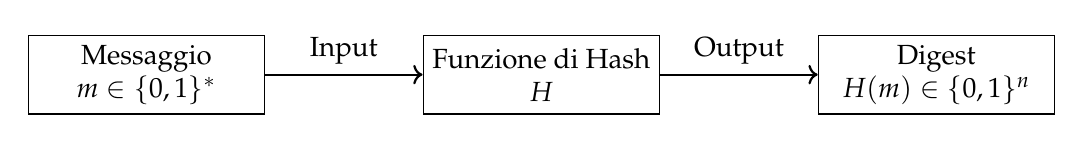
\begin{tikzpicture}[scale=1.5, every node/.style={scale=1}]
        
        % Input message 
        \node[draw, minimum width=3cm, minimum height=1cm, align=center] (input) {Messaggio \\ $m \in \{0,1\}^*$};
        % Hash function box 
        %\filldraw[draw=black, fill=blue!30, rotate=270] (4,0) -- (6,0) -- (5.5,1) -- (4.5,1) -- cycle; 
        \node[draw, minimum width=3cm, minimum height=1cm, align=center, right=2cm of input] (hash) {Funzione di Hash \\ $H$};
        % Digest (output) 
        \node[draw, minimum width=3cm, minimum height=1cm, align=center, right=2cm of hash] (output) {Digest \\  $H(m) \in \{0,1\}^n$};
        % Arrows 
        \draw[->, thick] (input) -- (hash) node[midway, above] {Input};
        \draw[->, thick] (hash) -- (output) node[midway, above] {Output};
        
        % Labels for security properties 
    \end{tikzpicture}
\end{figure}

\vspace{0.2cm}
\noindent
Le proprietà principali che sono richieste ad una funzione di questo dipo sono: 
\begin{itemize}
    \item devono essere progettate in modo tale che sia computazionalmente impraticabile invertire il processo detta anche \textbf{proprietà alle collisioni}, 
    \item una leggere variazione dell'input deve produrre un hash completamente diverso detta anche \textbf{proprietà di diffusione}.
\end{itemize}

Le funzioni di hash crittografiche sono utilizzate in molti contesti, tra cui: verifica di integrità, firma digitale e autenticazione.
Le funzioni di hash sono utilizzate per creare codici di autenticazione dei
messaggi (MAC) per garantire l'integrità e l'autenticità.

\subsection{Schemi crittografici}
Uno schema di cifratura è un insieme di algoritmi e funzioni che definisce come trasformare un messaggio in chiaro (plaintext) in un messaggio cifrato (ciphertext) e viceversa, al fine di garantire la confidenzialità e la sicurezza delle comunicazioni.
Formalmente possiamo rappresentarlo come una quintupla: 

\begin{center}
    \((\mathcal{P}, \mathcal{C}, \mathcal{K}, E, D)\)
\end{center}

\begin{itemize}
    \item \(\mathcal{P}\): Insieme dei messaggi in chiaro (plaintext).
    \item \(\mathcal{C}\): Insieme dei messaggi cifrati (ciphertext).
    \item \(\mathcal{K}\): Insieme delle chiavi utilizzate per la cifratura e decifratura,\textit{key space}.
    \item \(E: \mathcal{K} \times \mathcal{P} \to \mathcal{C}\): Funzione di cifratura.
    \item \(D: \mathcal{K} \times \mathcal{C} \to \mathcal{P}\): Funzione di decifratura.
\end{itemize}

\noindent
Deve esistere una relazione inversa tra le operazioni di cifratura e decifratura:
\begin{equation}
D(k, E(k, m)) = m \quad \forall m \in \mathcal{P}, \, k \in \mathcal{K}
\end{equation}

\begin{figure}[h!]
    \centering
    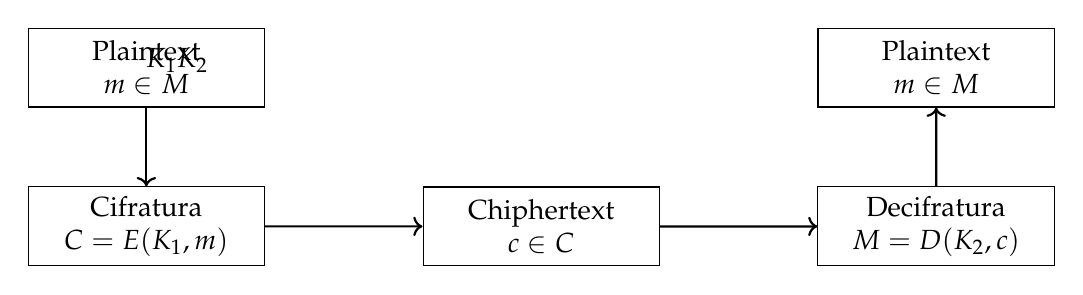
\begin{tikzpicture}[scale=1.5, every node/.style={scale=1}] 
    % Plaintext
    \node[draw, minimum width=3cm, minimum height=1cm, align=center] (plaintext) {Plaintext\\ $m \in M$};
    % Encryption box 
    \node[draw, minimum width=3cm, minimum height=1cm, below=1cm of plaintext, align=center] (enc) {Cifratura \\ $C = E(K_1,m)$};
    % Ciphertext 
    % se si riesce aggiungere delle linee di delimitazione che facciano intendere che in quesot modo il messaggio è protetto
    \node[draw, minimum width=3cm, minimum height=1cm, right=2cm of enc, align=center] (ciphertext) {Chiphertext\\ $c \in C$};
    % Decryption box 
    \node[draw, minimum width=3cm, minimum height=1cm, right=2cm of ciphertext, align=center] (dec) {Decifratura \\ $M = D(K_2,c)$};
    % Recovered message 
    \node[draw, minimum width=3cm, minimum height=1cm, above=1cm of dec, align=center] (plaintext2) {Plaintext\\ $m \in M$};
    
    % Arrows connecting the elements 
    \draw[->, thick] (plaintext) -- (enc) node[midway, above] {}; 
    \draw[->, thick] (enc) -- (ciphertext) node[midway, above] {}; 
    \draw[->, thick] (ciphertext) -- (dec) node[midway, above] {}; 
    \draw[->, thick] (dec) -- (plaintext2) node[midway, above] {};
    
    % Keys used for encryption and decryption 
    \drawkey{0,-2.1}{black}{$K_1$};
    \drawkey{6.8,-2.1}{black}{$K_2$};
    \end{tikzpicture}
    \label{fig:schema}
    \caption{Funzionamento di uno schema crittografico}
\end{figure}

\noindent
Lo schemo è descirtto in \textit{Fig. \ref{fig:schema}}, ed ha una defizione generale. Però se:
\begin{itemize}
    \item $K_1 = K_2$ allora si parla di un schema di crittografia simmetrico.
    \item $K_1 \neq K_2$ allora si parla di schema di crittografia asimmetrico.
\end{itemize}

\subsubsection{Simmetrici}

Come descritto poco fa, in uno schema simmetrico si utilizza la stessa chiave sia per le operazioni di cifratura che di decifratura. 
Significa che le due parti coinvolte nella comunicazione, devono possedere la stessa chiave segreta (PSK).\\
Gli utilizzi principali prevedono la cifratura dei dati, dato che è molto veloce, e in combinazione con funzioni di hash consente di ottenere codici HMAC

Alcuni esempi di crittosistemi simmetrici sono DES, AES,...



\subsubsection{Asimmetrici}

In uno schema di cifratura asimmetrica, detto anche a \textbf{chiave pubblica}, vengono utilizzate due chiavi distinte: una chiave pubblica e una chiave privata.
Lo spazio delle chiavi \(\mathcal{K}\) è costituito da una coppia di chiavi \((k_{\text{pub}}, k_{\text{priv}})\), dove:

\begin{itemize}
    \item \(k_{\text{pub}}\) è la chiave pubblica (usata per cifrare) 
    \item \(k_{\text{priv}}\) è la chiave privata (usata per decifrare)    
\end{itemize}

\noindent
Le due chiavi sono matematicamente legate, ma è computazionalmente difficile ottenere la chiave privata a partire da quella pubblica (questa è la base della sicurezza).
Quindi le due funzioni si riscrivono come:

\begin{equation}
    E: \mathcal{K}_{\text{pub}} \times \mathcal{P} \to \mathcal{C}
\end{equation}
\begin{equation}
    D: \mathcal{K}_{\text{priv}} \times \mathcal{C} \to \mathcal{P}
\end{equation}

Oltre alla classica cifratura, questa tipologia di schemi consente di realizzare due funzioni importanti, quello \textbf{firma digitale} e di \textbf{scambio di chiave}

Descrivere cosa è una firma, in particolare quella nel caso digitale e come viene utilizzata in combinazione con le funzione di hash per fare hash and sign\\

Oltre a questo poi parlare dello scambio di chiave ovvero l'utilizzo di crittografia asimmetrica per derivare un segreto condiviso tra le due parti.



\begin{figure}[htbp]
    \centering
    \begin{tikzpicture}[node distance=1.5cm]
        \node (entity1) [draw=green, rectangle] {Alice};
        \drawkey{-0.8, -0.8}{black}{$K_{pri}$};
        \drawkey{-1.6, -0.8}{black}{$K_{pub}$};
        \node (entity2) [draw=blue, rectangle, right=of entity1, xshift=3cm] {Bob};
        \draw (entity1) -- ++(0,-5) coordinate (vertical1);
        \draw (entity2) -- ++(0,-5);
        \draw[-stealth] (entity1) ++(0,-1) -- (entity2 |-,-1) node[midway, above, text=black, font=\footnotesize] {$K_{pub}$};
        \draw[stealth-] (entity2) ++(0,-2) -- (entity1 |-,-2) node[midway, above, text=black, font=\footnotesize] {$E(K_{pub},m)$};
    \end{tikzpicture}
    \label{}
    \caption{}
\end{figure}

\subsection{Confronto}

L'assunto che si è fatto in entrambi le tipologie di schema è che l'altra parte della comunicazione avesse ottenuto in qualche modo la chiave. Tuttavia la distribuzione
delle chiavi è un problema importante per il crittosistema ed ognuno ha le proprie caratteristiche. \\

\noindent
Se consideriamo le chiavi simmetriche abbiamo che all'aumentare degli host che vogliamo far comunicare ho bisogno di $n(n-1)/2$ chiavi, dove $n$ è il numero di terminali. Questo approccio è più robusto 
ma come possiamo vedere in \textit{Fig. \ref{fig:chiavi-simmetriche}} il problema porta ad un'esplosione combinatoria. Per questo motivo un approccio che limita questo 
fenomeno è quello del Key Distribution Center (KDC), che tuttavia rappresenta un'approccio centralizzato.
\begin{figure}
    \centering
    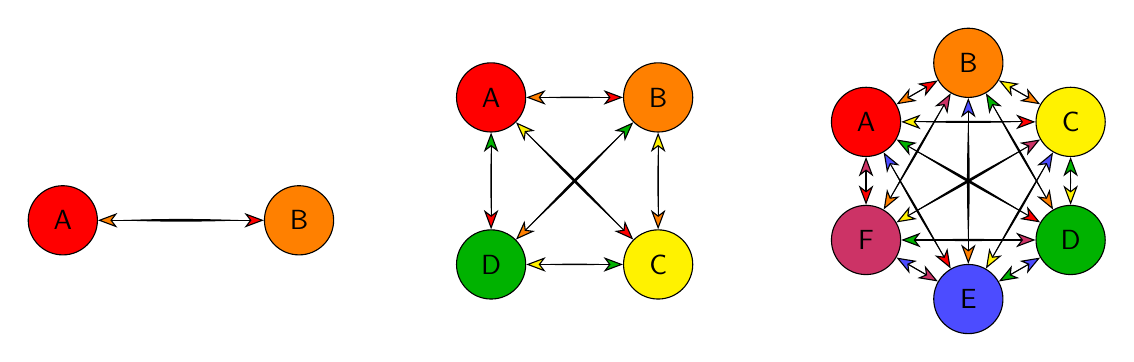
\begin{tikzpicture}[font=\sffamily,pics/cgram/.style={code={ \foreach \XX
        [count=\YY starting from 0] in {1,...,#1}
        {\pgfmathsetmacro{\mycolor}{{\LstCols}[\YY]} \node[circle,draw,minimum size=2.
        5em,fill=\mycolor] (c-#1-\XX) at ({{\LstAngles}[#1-2]-\YY*360/#1}:1.5)
        {\setcounter{pft}{\XX}\Alph{pft}};} \foreach \XX [evaluate=\XX as \Ymax using
        {int(\XX-1)}] in {2,...,#1} {\foreach \YY in {1,...,\Ymax}
        {\pgfmathsetmacro{\mycolorA}{{\LstCols}[\XX-1]}
        \pgfmathsetmacro{\mycolorB}{{\LstCols}[\YY-1]} \path (c-#1-\XX) -- (c-#1-\YY)
        coordinate[pos=0.1] (aux0) coordinate[pos=0.9] (aux1); \fill[black] (aux0)
        to[bend left=2] (aux1) to[bend left=2] (aux0); \draw[{Stealth[fill=\mycolorB,
        length=7pt,inset=2pt]}-{Stealth[fill=\mycolorA,length=7pt,inset=2pt]}]
        (c-#1-\XX) -- (c-#1-\YY); }}}}] \def\LstCols{"red","orange","yellow","green!70!
        black","blue!70!white","purple!80!white"} \def\LstAngles{180,150,135,128,150}
        \path (-5,0) pic {cgram=2} (0,0.5) pic {cgram=4} (5,0.5) pic {cgram=6}; 
    \end{tikzpicture}
    \label{fig:chiavi-simmetriche}
    \caption{Distribuzione delle chiavi simmetriche}
\end{figure}

Se invece andiao a considerare i crittosistemi a chiave pubblica abbiamo che questi si possono distribuire tramite certificati di chiave pubblica.
Questi tuttavia hanno bisogno di un'infrastruttura che li sorregge, questa è la PKI (Public Key Infrastructure).
Descrivere quelli che sono i componenti dell'infrastruttura e lo standard per la definzione dei certificati.

\subsection{Sicurezza}

Il \textbf{security level} è una misura della forza che una primitiva crittografica raggiunge rispetto ad attacchi.
Solitamente viene espresso come un numero di “bit di sicurezza”, dove $n$-bit di sicurezza significa che l'attaccante dovrebbe eseguire $2*n$ operazioni per romperlo.

Per i cifrari simmetrici, il \textit{livello di sicurezza} è pari alla dimensione del key-space. Mentre la sicurezza degli algoritmi asimmetrici si basa su problemi matematici che sono efficienti da calcolare in una direzione, ma inefficienti da invertire da parte dell'attaccante.
Tuttavia, gli attacchi contro gli attuali sistemi a chiave pubblica sono sempre più veloci della ricerca a forza bruta dello spazio delle chiavi.

Il NIST (National Institute of Standards and Technology) ha introdotto livelli di sicurezza per gli algoritmi di cifratura asimmetrica e post-quantistica come parte della sua iniziativa per standardizzare algoritmi che resistano anche ai computer quantistici.
I livelli sono definiti in \textit{Tabella \ref{tab:security-levels}}.

% NIST Security Level Table
\renewcommand{\arraystretch}{1.3} 
\begin{table}[ht]
    \centering
    \begin{tabular}{>{\centering\arraybackslash}m{3cm}p{10cm}}
        \hline
        \textbf{Security Level} & \textbf{Descrizione} \\
        \hline
        \textbf{Livello 1} & Sicurezza equivalente alla cifratura simmetrica con chiavi da 128 bit, come AES-128.\\
        \textbf{Livello 2} & Sicurezza equivalente ad attacchi contro SHA-256, con complessità circa pari a 128 bit. Leggermente più sicuro del livello 1. \\
        \textbf{Livello 3} & Sicurezza equivalente alla cifratura simmetrica con chiavi da 192 bit, come AES-192. \\
        \textbf{Livello 4} & Sicurezza equivalente ad attacchi contro SHA-384. Leggermente più sicuro del Livello 3. \\
        \textbf{Livello 5} & Sicurezza equivalente alla cifratura simmetrica con chiavi da 256 bit, come AES-256. \\
        \hline
    \end{tabular}
    \caption{Security Levels definiti dal NIST}
    \label{tab:security-levels}
\end{table}

\newpage
\section{Applicazioni}

Per loro natura le reti sono un mezzo di comunicazione non sicuro, essendo di tipo broadcast.
Nel contesto delle comunicazioni digitali, la crittografia gioca un ruolo fondamentale per garantire la sicurezza dei dati scambiati tra entità remote. 
I crittosistemi, ovvero applicazioni crittografica, combinano algoritmi di cifratura, autenticazione e gestione delle chiavi per garantire la riservetezza e l'integrità dei dati scambiati. 
Uno dei principali modelli di riferimento per la trasmissione di dati su Internet è il modello TCP/IP, che suddivide il processo di comunicazione in diversi livelli, ciascuno con funzioni specifiche.

% MODELLO TCP/IP
\begin{figure}[h!]
    \centering
    \includegraphics[scale=0.3]{Figures/security_tcp.png}
    \label{fig:tcpip}
    \caption{Modello TCP/IP con Protocolli di Sicurezza}
\end{figure}

Come mstrato in \textit{Fig. \ref{fig:tcpip}} possiamo fare sicurezza ai vari livelli della pila, ognuno con le proprie caratteristiche.
Tuttavia fare sicurezza a L3 ha il significativo vantaggio che tutti gli strati superiori convergono su di lui e dunque non è necessario andare a modifcare le singole applicazioni.
IPsec è una suite di protocolli i cui principali componenti, come mostrato in \textit{Fig. \ref{fig:ipsec-suite}}, sono: 

\begin{itemize}
    \item \textbf{AH}: Authentication Header, serve per avere integrità e autenticazione
    \item \textbf{ESP}: Encapsulating Security Payload, permette di rispettare tutti i requisiti di sicurezza
    \item \textbf{SA}: Security Association, è un insieme di parametri che definisce come i dati devono essere protetti durante la comunicazione tra due entità su una rete. Ogni SA contiene le informazioni necessarie per stabilire e mantenere una connessione sicura.
    \item \textbf{Algoritmi}: gli algoritmi crittografici e di hashing ausiliari per ottenere sicurezza
    \item \textbf{IKE}: Internet Key Exchange, si tratta di un protocollo utilizzato per negoziare, autenticare e distribuire dinamicamente le chiavi crittografiche utilizzate per proteggere le comunicazioni IPsec
\end{itemize}

\begin{figure}[!ht] 
    \centering 
    \scalebox{0.75}{
        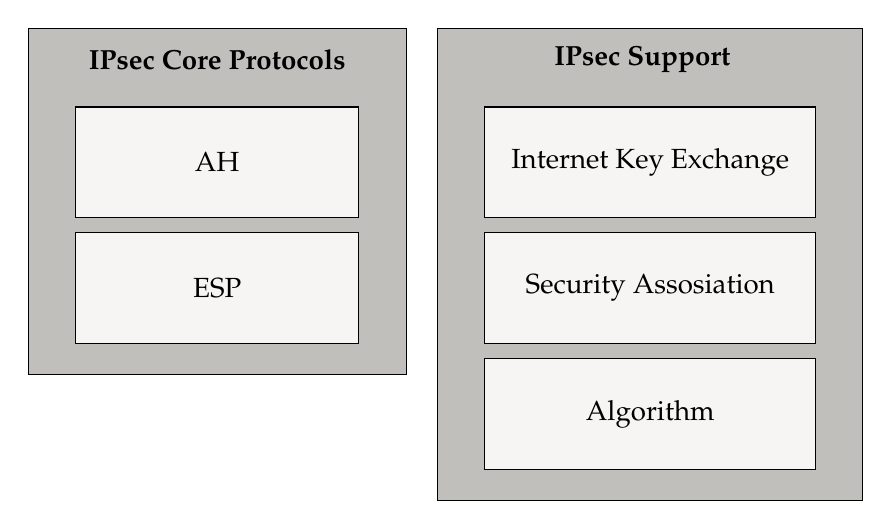
\begin{tikzpicture}[scale=0.8]
            \draw [ fill={rgb,255:red,192;green,191; blue,188} ] (5.5,13.25) rectangle (11.5,7.75); 
            \draw [ fill={rgb,255:red,246;green,245; blue,244} ] (6.25,10) rectangle node {ESP} (10.75,8.25); 
            \draw [ fill={rgb,255:red,192; green,191; blue,188} ] (12,13.25) rectangle (18.75,5.75); 
            \draw [ fill={rgb,255:red,246; green,245; blue,244} ] (6.25,12) rectangle node {AH} (10.75,10.25); 
            \node at (8.5,12.75) {\textbf{IPsec Core Protocols}}; 
            \node at (15.25,12.75) {\textbf{IPsec Support}}; 
            \draw [ fill={rgb,255:red,246; green,245; blue,244} ] (12.75,12) rectangle node { Internet Key Exchange} (18,10.25); 
            \draw [ fill={rgb,255:red,246; green,245; blue,244} ] (12.75,10) rectangle node { Security Assosiation} (18,8.25); 
            \draw [ fill={rgb,255:red,246; green,245; blue,244} ] (12.75,8) rectangle node { Algorithm} (18,6.25); 
        \end{tikzpicture}
    }
\label{fig:ipsec-suite} 
\caption{IPsec Protolocol Suite}
\end{figure}
\subsection{Security Association}

Le comunicazioni sicure si costruiscono sopra un concetto fondamentale noto come Security Association (SA). 



\subsection{IKE}


Il protocollo IKEv2, definito nell'\texttt{RFC 7296}, è un protocollo di rete che è responsabile della negoziazione di chiavi crittografiche e dei parametri di sicurezza tra due dispositivi, solitamente chiamati peer.

\begin{figure}[htbp]
    \centering
    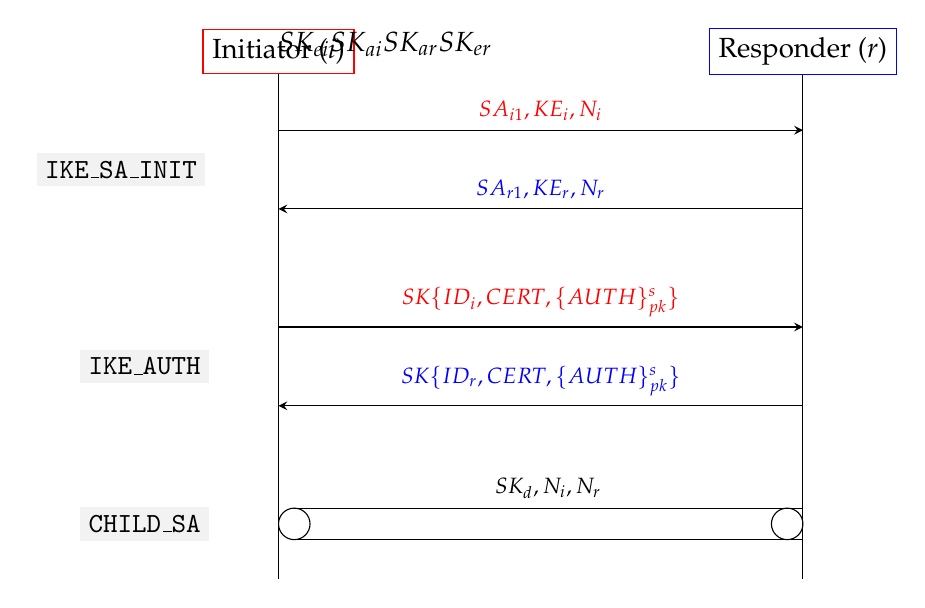
\begin{tikzpicture}[node distance=1.5cm]
        % Initiator and Responder
        \node (entity1) [draw=red, rectangle] {Initiator (\textit{i})};
        \node (entity2) [draw=blue, rectangle, right=of entity1, xshift=3cm] {Responder (\textit{r})};
        \draw (entity1) -- ++(0,-6.7) coordinate (vertical1);
        \draw (entity2) -- ++(0,-6.7);
        % IKE_INIT_SA
        \draw[-stealth] (entity1) ++(0,-1) -- (entity2 |-,-1) node[midway, above, text=red, font=\footnotesize] {$SA_{i1}, KE_i, N_i$};
        \draw[stealth-] (entity1) ++(0,-2) -- (entity2 |-,-2) node[midway, above, text=blue, font=\footnotesize] {$SA_{r1},KE_r,N_r$};
        % IKE_AUTH
        \draw[-stealth] (entity1) ++(0,-3.5) -- (entity2 |-,-3.5) node[midway, above, text=red, font=\footnotesize] {$SK\{ID_i, CERT, \{AUTH\}^s_{pk}\}$};
        \draw[stealth-] (entity1) ++(0,-4.5) -- (entity2 |-,-4.5) node[midway, above, text=blue, font=\footnotesize] {$SK\{ID_r, CERT, \{AUTH\}^s_{pk}\}$};
        % CHILD_SA 
        \node at (-1.7,-6) {\inlinecode{CHILD\_SA}};
        \node at (-2,-1.5) {\inlinecode{IKE\_SA\_INIT}};
        \node at (-1.7,-4) {\inlinecode{IKE\_AUTH}};
        \draw (entity1) ++(0.2,-6) ellipse (0.2cm and 0.2cm);
        \draw [-] (0.2,-6.2) -- (6.65,-6.2);
        \draw [-] (0.2,-5.8) -- (6.65,-5.8) node[midway, above, font=\footnotesize]{$SK_d, N_i, N_r$};
        \draw (entity2) ++(-0.2,-6) ellipse (0.2cm and 0.2cm);
        % Key for encryption and authtenticatoin
        \drawkey{-1, -2.3}{red}{$SK_{ei}$};
        \drawkey{-1.8, -2.3}{red}{$SK_{ai}$};
        \drawkey{8, -2.3}{blue}{$SK_{ar}$};
        \drawkey{8.8, -2.3}{blue}{$SK_{er}$};
        % Group
        \drawcurlybrace{0,-1}{0, -2}{};
        \drawcurlybrace{0,-3.5}{0, -4.5}{};
    \end{tikzpicture}
    \label{fig:ike_exchange}
    \caption{Fasi di Negoziazione del Protocollo IKEv2}
\end{figure}

Lo schema generale di funzionamento del protocollo al termine del quale i due hanno stabilito una SA è riportato in \textit{Fig. \ref{fig:ike_exchange}}.

\subsection{\textbf{IKE\_SA\_INIT}}

Lo scopo di questa prima fase è quello di creare una \textbf{IKE SA}, che consenta di rendere sicure i successivi scambi di dati al fine di realizzare una \textbf{IPsec SA}.
Dunque funge da apripista al fine di stabilire quelli che sono i parametri di sicurezza al fine di avere una comunicazione sicura. Per questo motivo in questo scambio i peer 
si scambiano le seguenti informazioni:

\begin{table}[htbp]
    \centering
    \caption{Tabella dei parametri e delle descrizioni}
    \begin{tabular}{ll}
        \toprule
        \textbf{Parametro} & \textbf{Descrizione} \\
        \midrule
        \textit{SA} & Security Association, vengono negoziati i parametri per la SA\\
        \textit{KE} & Key Exchange, e nel caso classico è l'esponente DH \\
        \textit{N} & Nonce \\
    \bottomrule
    \end{tabular}
\end{table}

\noindent
Al termine di questo scambio i due peer ottengono il \textit{DH Shared Secret} (indicato con $g^{ir}$), il quale insisme ai nonce, consentirà di ottenere 
quelli che sono i parametri di sicurezza della $IKE SA$ al fine di instauare un canale sicuro, per approfondimenti in \href{AppendixA}{appendice}.

% Tabella che riporta le varie funzioni delle chiavi

\subsection{IKE\_AUTH}

Il risultato della fase precedente è un canale sicuro su cui comunicare, in quanto è cifrato e utenticato. Si questo hanno luogo gli scambi per instaurare la IPsec SA.
In questa fase i nodi si autenticano mutuamente:

\begin{table}[htbp]
    \centering
    \caption{Tabella dei parametri e delle descrizioni}
    \begin{tabular}{ll}
        \toprule
        \textbf{Parametro} & \textbf{Descrizione} \\
        \midrule
        \textit{AUTH} & Payload che deve essere firmato affinchè ci sia autenticazione \\
        \textit{CERT} & Si allega il certificato digitale per la chiave pubblica \\
        \textit{CERTQ} & Si fa richiesta al peer di fornire il certificato \\
    \bottomrule
    \end{tabular}
\end{table}

Tutto il contenuto appena descritto è protetto mediante le chiavi segrete di quella direzione. Ciò è indicato mediante la notazione $SK\{...\}$
La modalità di autenticazione può essere: PSK, EAP oppure mediante chiave pubblica.

\subsection{CHILD\_SA}


\section{Problemi}

IKEv2 utilizza come porotocollo a livello trasporto UDP per per inoltrare i propri messaggi. La maggior parte dei messaggi che i peer si scambiano hanno dimensioni relativamente piccole e
quindi che non eccedono l'\textbf{MTU} di un pacchetto IP, tuttavia abbiamo degli scambi che richiedono un trasferimento di dati abbastanza grandi.

Per esempio nel caso di autenticazione tramite pubkey nella fase di \inlinecode{IKE\_AUTH} è necessario trasferire il proprio certificato che in base allo schema di firma utilizzato
può arrivare anche a diversi Kbyte di dimensione. In questi casi si verifica la frammentazione a livello IP.

%Immagine frammentazione

\begin{figure}[htbp]
    \centering
    \begin{tikzpicture}[node distance=2cm,>=Latex]
        % Nodi
        \node (initiator) [client] {Initiator};
        \node (device) [router, right=of initiator] {Device};
        \node (responder) [client, right=of device] {Responder};
        \node (message) [messageclosed, fill=orange!40, minimum size=0.6cm] at (1.9,0.5) {};
        \node (message2) [messageclosed, fill=gray!40, minimum size=0.6cm] at (1.2,0.5) {};
        \node (drop) [messageclosed, fill=gray!40, minimum size=0.6cm, , font=\small, text=red] at (3,1) {};
        \node (message3) [messageclosed, fill=orange!40, minimum size=0.6cm, , font=\small, text=red] at (4.5,0.5) {};

        \draw[-] (initiator.east) -- (device.west);
        \draw[-] (device.east) -- (responder.west);

    \end{tikzpicture}
    \vspace*{1cm}
    \caption{Drop Pacchetti}
    \label{fig:cgnatdrop}
\end{figure}

Diversi test hanno mostrato che nel caso in cui i peer si trovino in presenza di CGNAT potrebbero non istausarsi le SA. Questo è dovuto al fatto che i device degli ISP non
consentono ai frammenti IP di passare attravers di loro, ovvero scartano i pacchetti e di conseguenza bloccano le comunicazioni IKE.
Questo è riportato schematicamente in Fig. \ref{fig:cgnatdrop}.
Questo drop dei pacchetti avviene perchè esistono numerosi vettori di attacco che fanno affidamento sulla frammentazione IP, per questo motivo gli ISP operano un filtro su questa tipologia di pacchetti.
Ance se in teoria uno dei requisiti del CGNAT definito dagli RFC è proprio consentire la frammentazione.

Per risolvere questa problematica e dunque consentire il passaggio dei messaggi attraverso i dispositivi di rete che non consentono il passaggio degli IP fragment attraverso 
di loro nell' RFC 7283 viene introdotta la IKEv2 \textit{Message Fragmentation}. In cui la frammentazione dei messaggi è gestita direttamente da parte di chi implementa IKEv2

\subsection{\inlinecode{IKE\_INTERMEDIATE}}

Per evitare che nel trasferimento di grandi dati ciò avvenga viene introdotto uno scambio aggiuntivo. Questo scambio è introdotto per quei casi in cui la dimensione dei dati
da trasferire ecceda la dimensione massima che causerebbe la frammentazione IP. Questo scambio va fatto dopo la \inlinecode{IKE\_INIT\_SA} e prima della \inlinecode{IKE\_AUTH} in questo
modo è sia autenticato che cifrato tramite le chiavi negoziate dal primo scambio.

\begin{figure}[htbp]
    \centering
    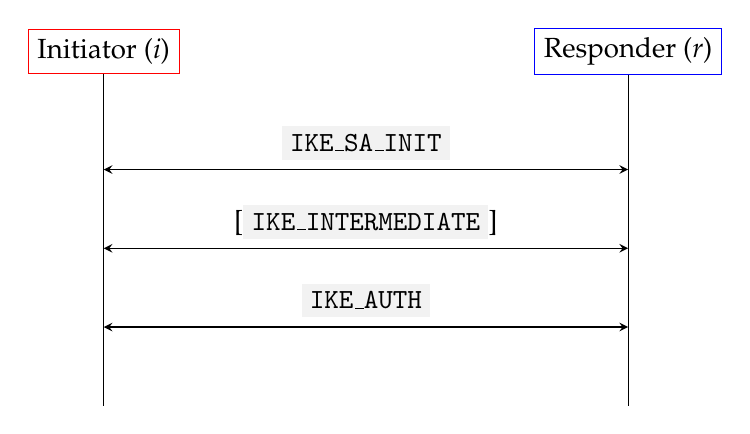
\begin{tikzpicture}[node distance=1.5cm]
        % Initiator and Responder
        \node (entity1) [draw=red, rectangle] {Initiator (\textit{i})};
        \node (entity2) [draw=blue, rectangle, right=of entity1, xshift=3cm] {Responder (\textit{r})};
        \draw (entity1) -- ++(0,-4.5) coordinate (vertical1);
        \draw (entity2) -- ++(0,-4.5);
        % IKE_AUTH
        \draw[stealth-stealth] (entity1) ++(0,-1.5) -- (entity2 |-,-1.5) node[midway, above] {\inlinecode{IKE\_SA\_INIT}};
        \draw[stealth-stealth] (entity1) ++(0,-2.5) -- (entity2 |-,-2.5) node[midway, above] {[\inlinecode{IKE\_INTERMEDIATE}]};
        \draw[stealth-stealth] (entity1) ++(0,-3.5) -- (entity2 |-,-3.5) node[midway, above] {\inlinecode{IKE\_AUTH}};
    \end{tikzpicture}
    \caption{Scambio nuovo}
    \label{fig:ikeintermediate}
\end{figure}

Questo scambio è posizionato qui in quanto nella \inlinecode{IKE\_SA\_INIT} per motivi di sicurezza non è possibile applicare la frammentazione.
Di solito i messaggi sono piccoli abbastanza da non causare la frammentazione IP, tuttavia questo potrebbe cambiare se si utilizzano scambi di chiave QC-resistant; in quanto
hanno chiavi pubbliche larghe e che quindi causerebbero frammentazione IP.

Per questo viene aggiunto questo scambio che viene utilizzato per trasferire grandi quantità di dati.

L'utilizzo principale di questo scambio è quello di trasferire le chiavi pubbliche QC-resistant, tuttavia in generale può essere utilizzzato per trasferire qualsiasi tipologia di dato.
Quindi il principale utilizzo è quello di fare un \textbf{enforcing} delle chiavi negoziate tramite DH al fine di renderle QC-resistant. Infatti se durante questo scambio si scambiano 
altre chiavi allora le coppie $\{SK_{a[i/r]}, SK_{e[i/r]}\}$ vengono aggiornate.

Permette di realizzare Multiple Key Exchange
Gli scambi di chiave aggiuntivi vengono aggiunti alla proposal tramite \inlinecode{PQ\_KEM\_1}



Lo scambio \inlinecode{IKE\_FOLLOWUP\_KE} è introdotto specificatamente per trasferire dati sulla chiavi addizionali da realizzare in una CHILD SA.
In questo caso le chiavi aggiuntive vengono utilizzate per aggiornare il KEYMAT



\begin{itemize}
    \item flag \inlinecode{IKE\_FRAGMENTATION\_SUPPORT}: il peer dice di supportare la frammentazione IKEv2, affinchè venga utilizzata entrambi i peer devono supportarla.
    \item flag \inlinecode{INTERMEDIATE\_EXCHANGE\_SUPPORT}: il peer dice di supportare gli scambi intermedi
\end{itemize}

Una volta terminati gli scambi, per proteggere lo scambio \inlinecode{IKE\_AUTH} e gli scambi successivi vengno utilizzata le ultime chiavi calcolate
Dato che i dati trasferiti in questi scambi aggiuntivi vanno autenticati si aggiungono all'\inlinecode{AUTH} payload che poi andrà 



Il supporto per lo scambio aggiuntivo viene comunicato aggiungendo all'interno
dell \inlinecode{IKE\_SA\_INIT} il flag \inlinecode{IKE\_INT\_SUP} (che sta per
Intermediate Exchange Support).
Se anche il responder lo supporta lo includerà nel messaggio di risposta dello
scambio.




Considerazioni, L'IKE fragmentation viene introdotta a causa del NAT tuttavia nel nostro caso di satelliti non ha senso utilizzarla in quanto non credo che si utilizzi
il NAT soprattutto perchè introduce ritardi dovuti alla traduzione degli indirizzi



\section{Post-Quantum}

Un solo KEM con Kyber L1 usando come suite AES\_GCM has vabene come certificato dilithium L1

Nel KEM quanti cifrano?

Cioè l'initiator manda il certificato e poi il responder cifra 
 
% Chapter Template

\chapter{Scenario} % Main chapter title

\label{Chapter3} % Change X to a consecutive number; for referencing this chapter elsewhere, use \ref{ChapterX}

\textit{In questo capitolo facciamo un introduzione su quello che è lo scenario che stiamo considerando per il nostro lavoro: 
quello delle comunicazioni satellitare. Vediamo nel dettaglio quali sfide introduce, le tecnologie utilizzate 
e come affrontare le possibile problematiche a causa di applicare la PQC.}

%----------------------------------------------------------------------------------------
%	SECTION 1
%----------------------------------------------------------------------------------------

\section{Comunicazioni Satelliari}


Le comunicazioni satellitari sono fondamentali per le infrastrutture moderne, poichè abilitano una vasta gamma di servizi.
Negli ultimi decenni, con l'aumento della domanda di connettività globale e l'espansione delle reti di comunicazione, i satelliti sono diventati strumenti essenziali per garantire una copertura estesa.
L'emergere delle costellazioni di satelliti in orbita bassa (LEO - Low Earth Orbit) sta cambiando il paradigma delle comunicazioni satellitari, offrendo vantaggi significativi rispetto ai satelliti geostazionari (GEO), un confronto tra le due orbite è mostrato in \textit{Figura \ref{fig:orbite}}. 
%Mentre i satelliti GEO forniscono una copertura stabile, i satelliti LEO consentono Round Time Trip (RTT) notevolmente ridotti e una maggiore flessibilità, rendendoli ideali per applicazioni ad alta velocità come la trasmissione dati in tempo reale e la connettività Internet globale.
\todo{Scrivere meglio questa parte finale}
Questo cambio di paradigma insieme al quantum computer hanno portato diversi enti, tra cui l'Agenzia Spaziale Europea (ESA), ad affrontare nuove sfide.

\begin{figure}[h!]
    \centering
    \begin{tikzpicture}
        % Definizione dei colori per le orbite
        \definecolor{leo}{gray}{0.2}    % Grigio scuro
        \definecolor{geo}{gray}{0.1}% Grigio molto scuro
        \definecolor{terra}{HTML}{008F39}
        \node at (-4.8, 0) [color=geo]{GEO};
        \node at (3.5, 0) [color=leo]{LEO};
        \node at (0, 0) {Terra};
        
        \draw[thick, dashed, geo] (0,0) circle (4.2cm);
        \draw[thick, dashed, leo] (0,0) circle (3cm);
        \filldraw[fill=mare,] (0,0) circle (2.2cm);

        \path[draw, decoration={text along path, text={$2.000km$}, text align=center}, decorate] (0,0) (180:2.8cm) arc (180:360:2.8cm);
        \path[draw, decoration={text along path, text={$36.000km$}, text align=center}, decorate] (0,0) (180:4cm) arc (180:360:4cm);

        \node at (-2.5,2) {\includegraphics[width=1cm]{Figures/satellite.png}}; % Sostituisci 'your_image.png' con il percorso della tua immagine
        \node at (3.2,3) {\includegraphics[width=1cm, angle=270]{Figures/satellite.png}}; % Sostituisci 'your_image.png' con il percorso della tua immagine
        \node at (0.2,0.5) {\includegraphics[width=3cm ]{Figures/europe.png}}; % Sostituisci 'your_image.png' con il percorso della tua immagine

        \node[cloud, cloud puffs=15.7, cloud ignores aspect, minimum width=1.5cm, minimum height=0.5cm, align=center, fill=white, draw] (cloud) at (-2, 0) {};
        \node[cloud, cloud puffs=15.7, cloud ignores aspect, minimum width=1.5cm, minimum height=0.5cm, align=center, fill=white, draw] (cloud) at (2, -0.5) {};

    \end{tikzpicture}
    \caption{Orbite dei satelliti}
    \label{fig:orbite}
\end{figure}

\subsection{Limitazioni}

L'ambiente spaziale, caratterizzato da radiazioni intense, temperature estreme e lunghi periodi senza manutenzione, pone sfide significative in termini di progettazione e operatività dell'hardware e del software.
Tra i principali vincoli per l'hardware satellitare troviamo:

\begin{itemize}
    \item \textit{Resistenza alle radiazioni}: i componenti elettronici sono progettati per resistere all'esposizione costante alle radiazioni spaziali.
    \item \textit{Basso consumo energetico}: l'energia disponibile per le operazioni risulta limitata, quindi si usano processori a basso consumo e ad alta efficienza energetica, sacrificando potenza di calcolo.
    \item \textit{Elaborazione in tempo reale}: per alcune tipologie di servizi è necessario che il processamento avvenga in tempo reale.
    \item \textit{Compattezza}: a causa dello spazio limitato a bordo di un satellite, i componenti hardware devono essere progettati in modo estremamente compatto.
\end{itemize}

\noindent
L'hardware limitato ha un impatto diretto sullo sviluppo del software per i satelliti. 
Rispetto al un contesto terrestre, dove le risorse computazionali sono abbondanti, il software per i satelliti deve essere ottimizzato per funzionare su processori con bassa potenza di calcolo e memoria ridotta. 
Le principali sfide per gli sviluppatori sono:

\begin{itemize}
    \item \textit{Semplicità e ottimizzazione}: gli algoritmi devono essere semplici e ottimiz\-zati per funzionare su hardware con risorse limitate.
    \item \textit{Parallelismo limitato}: le operazioni devono essere eseguite in modo lineare o con limitato parallelismo, aumentando la complessità della progettazione.
    \item \textit{Affidabilità assoluta}: il software deve essere robusto, sicuro e testato ampiamente in modo tale che possibile errori non abbiano conseguenza catastrofiche.
\end{itemize}

\noindent
È fondamentale prestare particolare attenzione alle implementazioni 
crittogra\-fiche dato che in contesto come questo, risulta cruciale trovare un equilibrio tra
sicurezza e prestazioni. Da un lato, è necessario proteggere le comunicazioni
utilizzando algoritmi crittografici complessi; dall'altro, è essenziale
garantire che le operazioni eseguite non compromettano l'operatività del
satellite.

\subsection{Stato Attuale}

Per capire quale è la differenza in termini di hardware e software rispetto a quelli a cui siamo abiutati 
introduciamo quelli che sono gli attuali standard impiegati in questo settore.

\begin{itemize}
    \item Tra i processori utilizzati abbiamo \textit{LEON3}, un processore open-source basato sull'architettura SPARC, progettato dall'ESA. 
    \item ESA Power Interface Standard (ECSS-E-ST-20C): definisce come deve avvenire la distribuituzione dell'alimentazione elettrica all'interno dei satelliti.
    \item Cubesat Standard: definisce dimensioni compatte modulari (10x10x10 cm per 1U) per ridurre i costi e semplificare il lancio e la costruzione dei satelliti.
    \item Triple Modular Redundancy (TMR): nei sistemi critici spaziali si utilizza la ridondanza tripla modulare, per garantire l'affidabilità dei risultati tramite sistemi di voting.
\end{itemize}
\noindent
Il sistema operativo utilizzato in queste applicazioni è RTEMS (Real-Time Executive for Multiprocessor Systems) che le caratteristiche di essere open-source, real-time e basato su GNU/Linux.
\todo{se si trova riportare qualche riferimento}

%-----------------------------------
%	SECTION 2
%-----------------------------------
\subsection{Sfide}
\noindent
Per rendere le comunicazioni satellitari sicure ad attacchi Qauntum occorre adottare algoritmi più complessi.
Questi utilimi, tuttavia, oltre a richiedere più memoria per la gestione delle chiavi,
comportano un incremento significativo del carico di calcolo. Le sfide da affrontare sono:

\begin{itemize}
    \item  Aumento complessità computazionale: l'incremento delle dimensioni delle chiavi e della complessità degli algoritmi portano a un aumento del carico computazionale. Aggiungendo ulteriori vincoli su sistemi già limitati. 
    \item Incremento della larghezza di banda necessaria: oltre all'aumento di carico si ha anche magiore utilizzo della larghezza di banda, che in comunicazioni satellitari risuta già limitata.
    \item Compatibilità retroattiva: occorre adottare soluzioni ibride, in cui
    algo\-ritmi crittografici classici coesistono con quelli post-quantum. Questo a 
    causa dell'eterogeneità delle capacità dei satelliti in orbita.
\end{itemize}

\section{Benchmarking}

Per valutare l'applicabilità degli algoritmi di PQC
nel contesto satellitare, è fondamentale comprendere il loro impatto sui
protocolli di comunicazione. Inizialmente, analizzeremo tali algoritmi in un
ambiente desktop confrontan\-doli con quelli classici per evidenziare eventuali
differenze. Se le discrepanze risultano già significative nel contesto simulato,
sarà poco sensato considerarli in un ambiente ancora più limitato.


\subsection{Ambiente}

\begin{comment}
    L'ambiente di test, descritto in \textit{Tabella \ref{tab:env}}, è stato progettato in modo da isolare i singoli servizi all'interno di
    container, facilitando l'analisi del carico e delle risorse consumate da ciascuno di questi. 
\end{comment}

Il protocollo che consideriamo è IPsec, con un focus particolare sulla sua
implementazione in StrongSwan. Questa scelta è motivata dal fatto che StrongSwan
opera a un livello più basso dello stack TCP/IP, risultando così uno dei
protocolli più diffusi. L'implementazione delle primitive post-quantum è fornita dalla libreria \texttt{liboqs}. 
Questa fa parte del progetto open-source \textit{OpenQuantumSafe} (OQS).
Il quale a rendere disponibile l'infrastruttura crittografica necessaria per proteggere i sistemi informatici
dall'avvento dei computer quantistici. L'obiet\-tivo del progetto è quello di fornire:

\begin{itemize}
    \item API standardizzate per supportare lo scambio chiavi e la firma digitale. 
    \item Modularità, facilitando l'aggiunta di nuovi algoritmi. 
    \item Prestazioni ottimizzate per diverse architetture hardware.
\end{itemize}


\begin{table}[htbp] 
    \centering 
    \begin{tabular}{p{4cm} p{8cm}} 
        \toprule
        \textbf{Componente} & \textbf{Descrizione} \\ 
        \midrule
        \textbf{Hardware} & \\ 
        CPU & Ryzen 7-5825U (8 core, 3.8 GHz) \\ 
        RAM & 24 GB DDR4 \\ 
        Storage & 1024 GB SSD NVMe \\ 
        \textbf{OS} & \\ 
        Distribuzione & Arch Linux \\
        Kernel & Linux 6.10.10-arch1-1 \\ 
        \textbf{Software} & \\ 
        Linguaggio & Bash Script \\
        Strongswan & 6.0.0beta Post-Quantum IKEv2 Daemon \\
        liboqs & Version 0.9.2 \\
        Docker & Version 24.0.6 \\ 
        \hline 
    \end{tabular} 
    \caption{Descrizione dell'ambiente di test virtualizzato} 
    \label{tab:env}
\end{table}



\noindent
Si tratta di una raccolta di implementazioni di algoritmi crittografici post-quantum, KEM e SIG, e strumenti per integrarli in protocolli di sicurezza esistenti per sperimentare e testare il loro impatto.
In \textit{Tabelle \ref{tab:env}} è presente una descrizione dettagliata dell'ambiente utilizzato per fare i test.


\subsection{Metodologia}

Per ragioni progettuali e di portabilità del codice, il servizio Strongswan è stato 
containerizzato tramite l'utilizzo di Docker. Ciò consente di avere due istanze dello stesso
servizio in esecuzione contemporaneamente che comunicano attaverso un'interfaccia virtuale. 

\begin{center}
    \begin{verbatim}
            +-------+                         +--------+ 
            | carol | === Virtual Interf. === |  moon  |
            +-------+                         +--------+ 
    \end{verbatim}
\end{center}

\noindent
In secondo luogo siamo andati a definire quali sono le configurazioni da confrontare, riportate in 
\textit{Tabella \ref{tab:cipher_suites}}, ognuna delle quali è caratterizzata da:

\begin{itemize}
    \item \textbf{Chiper suite}: un'insieme di algoritmi crittografici che determinano la sicurezza di una connessione in un protocollo di rete.
    Le cipher suite sono generalmente denominate seguendo una convenzione di naming standardizzata che riflette i componenti inclusi nella suite.
    \begin{center}
        \texttt{<ENCR>\text{-}<INTEG>\text{-}<KEM>}
    \end{center}

    \item \textbf{Authentication Method}: sono supportati diverse modalità di autentica\-zione, tuttavia noi vogliamo vedere
    come si comportano gli schemi di firma post-quantum. Per questo motivo utilizzeremo l'autenticazione mediante 
    certificati. \todo{rimandare in appendice per il concetto di chain e root}
\end{itemize}

\noindent
Nella nostra analisi, abbiamo scelto tre configurazioni distinte per le cipher
suite, ognuna progettata per affrontare specifici aspetti delle tecnologie
critto\-grafiche attuali e future.

\noindent
La prima configurazione utilizza esclusivamente di \textit{primitive classiche}. 
Questa scelta rappresenta il benchmark attuale delle tecnologie di crittografia e fornisce una base
solida per confrontare le altre configurazioni. La seconda
configurazione è composta da \textit{primitive post-quantum}, e consente di
analizzare le prestazioni e l'efficacia delle soluzioni crittografiche
post-quantum nel contesto del protocollo. Infine, abbiamo implementato
una \textit{onfigurazione Ibrida}, la quale combina elementi delle primitive
classiche e post-quantum. Questa scelta è progettata per garantire la transizione 
graduale verso l'utilizzo esclusivo di tecnologie quantistiche.

\begin{comment}
    
    \begin{itemize}
    \item \textit{Configurazione Classica}: questa scelta rappresenta il benchmark attuale delle tecnologie
    di crittografia e fornisce una base solida per confrontare le altre configurazioni.
    \item \textit{Configurazione PQ}: questa configurazione permette di
    analizzare le pres\-tazioni e l'efficacia delle soluzioni crittografiche
    post-quantum nel conte\-sto del protocollo.
    \item \textit{Configurazione Ibrida}: questa configurazione è progettata
    per garantire una transizione verso il solo utilizzo di tecnologie
    quantistiche. 
\end{itemize}
\end{comment}

\renewcommand{\arraystretch}{1.2}
\todo{gli altri algoritmi tipo hqc, bike,...}
\begin{table}[h]
    \centering 
    \begin{tabular}{cll} 
        \toprule
        \textbf{Name} & \textbf{Chiper Suites} & \textbf{Firma Digitale}\\ 
        \midrule 
        \texttt{A1} & \texttt{aes128ctr\text{-}sha256\text{-}ecp256} & \texttt{ECDSA}         \\          
        \texttt{B1} & \texttt{aes128ctr\text{-}sha256\text{-}kyber1} & \texttt{dilithium2}                 \\ 
        \texttt{C1} & \texttt{aes128ctr\text{-}sha256\text{-}ecp256\text{-}ke1\_kyber1} & \texttt{falcon512} \\ 
        \hline
        \texttt{A3} & \texttt{aes192ctr\text{-}sha384\text{-}ecp384}         &  \texttt{ECDSA}        \\ 
        \texttt{B3} & \texttt{aes192ctr\text{-}sha384\text{-}kyber3}          &  \texttt{dilithium3}      \\ 
        \texttt{C3} & \texttt{aes192ctr\text{-}sha384\text{-}ecp384\text{-}ke1\_kyber3} & \texttt{falcon1024} \\
        \hline
        \texttt{A5} & \texttt{aes256ctr\text{-}sha512\text{-}ecp521}              &  \texttt{ECDSA}    \\ 
        \texttt{B5} & \texttt{aes256ctr\text{-}sha512\text{-}kyber5}               &  \texttt{dilithium5}   \\ 
        \texttt{C5} & \texttt{aes256ctr\text{-}sha512\text{-}ecp521\text{-}ke1\_kyber5} & \texttt{falcon1024} \\  
        \hline
    \end{tabular}
    \caption{Cipher Suites suddivise per Livello di Sicurezza} 
    \label{tab:cipher_suites} 
\end{table}


\noindent
Il testing viene realizzato attraverso uno script Bash. Nella Figura 3.2 è
illustrata la struttura dei file necessari per automatizzare l'intero processo,
consentendo così un'operazione completamente "zero-touch", che riduce al
minimo l'intervento manuale.
Tra questi abbiamo:

\todo{dire di fare riferimento in appendice?}

\begin{itemize}
    \item \texttt{Dockerfile}: a partire da un'immagine Ubuntu si installa il servizio StrongSwan e si integra la libreria liboqs.
    \item \texttt{docker-compose}: consente di orchestrare i due container, in cui si specifi\-cano volumi e parametri di connessione tra i due.
\end{itemize}
\noindent
Ad ogni container è associato a un volume, identificato con il proprio
nome, che contiene le configurazioni specifiche (connessioni e certificati) per il daemon.
Questa struttura facilita la modifica e il testing delle diverse configu\-razioni
senza influenzare l'altro container, contribuendo a un ambiente di test più
controllato e flessibile.

\noindent
Per automatizzare il processo di testing e garantire un'esecuzione efficiente, è
stato sviluppato uno script in Bash che gestisce l'intero flusso operativo.
Questo script si basa esclusivamente su utility integrate di Linux, eliminando
la necessità di installare software aggiuntivo. Esso non solo avvia i container
e configura i parametri necessari, ma si occupa anche della raccolta e
dell'analisi dei risultati. In \textit{Figura \ref{fig:flow}} è riportato il suo diagramma di flusso
in particolare le principali fasi.
\todo{dire di fare riferimento all'appendice per una descrizione dettagliata}
\todo{descrivere quelli che sono i principali tool utilizzati?}


\begin{figure}
    \dirtree{% 
    .1 /. 
    .2 \textcolor{blue}{carol}. 
    .3 \textcolor{blue}{conn}. 
    .3 swanctl.conf. 
    .3 \textcolor{blue}{x509}. 
    .3 \textcolor{blue}{x509ca}. 
    .2 \textcolor{green!80}{docker-compose.yml}. 
    .2 Dockerfile. 
    .2 \textcolor{blue}{moon}. 
    .3 \textcolor{blue}{conn}. 
    .3 swanctl.conf. 
    .3 \textcolor{blue}{x509}. 
    .3 \textcolor{blue}{x509ca}. 
    .2 strongswan.conf. 
    .2 \textcolor{green!90}{strongswan.sh}. 
    }
    \caption{Struttura delle directory}
    \label{fig:tree}
\end{figure}

\begin{figure}[h!]
    \centering
    \begin{tikzpicture}[node distance=2cm, scale=0.8]
        % Definizione dei blocchi 
        \tikzset{
            customnode/.style={rectangle, draw, minimum width=3cm, minimum height=1cm, inner sep=5pt},
            decisionnode/.style={diamond, draw, aspect=2, minimum width=3cm, inner sep=5pt}
        }
        \node (start)  [customnode, rounded corners] {Inizio}; 
	    \node (param1) [customnode, left=of start] {Conn: <nome>}; 
	    \node (param2) [customnode, right=of start] {Iterazioni: <num>}; 
        \node (docker) [below of=start, customnode] {Avvio ambiente}; 
        \node (config) [below of=docker, customnode] {Avvio della Conn};
        \node (sniff)  [below of=config, customnode] {Sniffing su interfaccia virtuale}; 
        \node (parsing)  [below of=sniff, customnode] {Parsing pacchetti e tempi}; 
        \node (condition) [below of=parsing, decisionnode] {Iterazioni=0}; 
        \node (result)  [below of=condition, customnode] {Stampa dei risultati}; 
        \node (end) [customnode, rounded corners, below of=result] {Fine};
        \draw [-, dashed] (param1) -- (start); 
        \draw [-, dashed] (param2) -- (start); 
        \draw [->] (start) -- (docker); 
        \draw [->] (docker) -- (config); 
        \draw [->] (config) -- (sniff);     
        \draw [->] (sniff) -- (parsing); 
        \draw [->] (parsing) -- (condition); 
        \draw [->] (condition) -- node[right]{Sì} (result);
        \draw [->] (result) -- (end);
        \draw [->, rotate=270] (condition.east) -- node[above]{No} ++(0,4)  -| (config.east);
    \end{tikzpicture}
    \caption{Diagramma di flusso dello script}
    \label{fig:flow}
\end{figure}

\subsection{Risutlati}

Le metriche di maggiore interesse, per il nostro studio, sono:

\begin{itemize}
    \item \textit{Tempo Complessivo} per stabilire la SA tra i due, il tempo di elabora\-zione del singolo algoritmo non ci interessa dato che ampiamente descritte
    dalla libreria openquantumsafe.   
    \item \textit{Packet Size} che rappresenta la quantità di dati scambiati
    tra i due nodi necessari per stabilire una Security Association (SA)
\end{itemize}

Ora riportiamo i grafici

\todo{grafico riassuntivo che riporta il confronto tra le varie configurazioni, uno per i tempi e uno per i pacchetti}

\begin{figure} 
    \centering 
    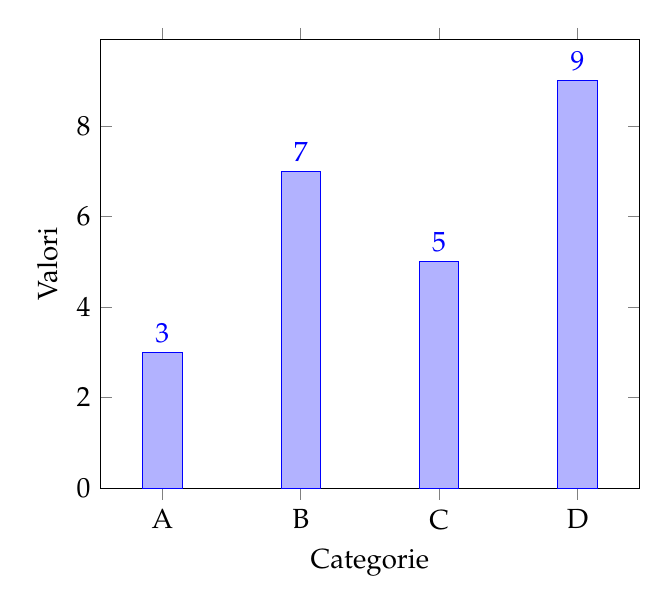
\begin{tikzpicture} 
        \begin{axis}[ 
            ybar, % Grafico a
            symbolic x coords={A, B, C, D}, % Etichette sull'asse x
            xtick=data, % Etichette dell'asse x corrispondono ai dati 
            ymin=0, % Valore
            ylabel={Valori}, % Etichetta dell'asse y 
            xlabel={Categorie}, 
            bar width=0.5cm, % Larghezza delle barre 
            nodes near coords,
            enlarge x limits=0.15 % Spazio aggiuntivo agli estremi
        ] 
        \addplot coordinates {(A,3) (B,7) (C,5) (D,9)}; 
        \end{axis}
    \end{tikzpicture} 
    \caption{Esempio di istogramma con dati fittizi.} 
\end{figure}


\newpage
\section{Tuttavia}

Notiamo che non ci sono enormi differenze in termini di tempi ma è presente un 
notevole aumento in termini della dimensione in particolare per quanto riguarda l'autenticazione.
E in contesto di questo tipo non è auspicabile

Cercando di trovare possibili soluzioni, ci siamo imbattuti su quello che è minimal IKE ovvero
una versione di IKE applicabile in scenari soggetti a constraint di risorse simili a quelli presenti nello spazio.

Riguardo a questo non esistono implementazioni, per questo motivo siamo passati a provare a dare un'implementazione di quest'ultimo
In modo tale che rappresenti un punto di inizio per questo scenario

Di questo trattiamo nel prossimo capitolo

%-----------------------------------
%	SECTION 3
%-----------------------------------


% Chapter Template

\chapter{Hummingbird} % Main chapter title

\label{ChapterX} % Change X to a consecutive number; for referencing this chapter elsewhere, use \ref{ChapterX}

%----------------------------------------------------------------------------------------
%	SECTION 1
%----------------------------------------------------------------------------------------

\section{Progettazione}

\subsection{Requisiti}

Nella parte di progettazione portare quelli che sono i requisiti che deve rispettare l'implementazione
sia funzionali che non
uno tra tutto met

\subsection{Architettura}

Archietettura sia delle directory che a livello dei moduli 
Il C richiede una chiara strutturazione per gestire la complessità del codice in modo efficace

\subsubsection*{Moduli}

Per mantenere la separazione dei compiti

\subsubsection*{Strutture Dati}

%-----------------------------------
%	SECTION 2
%-----------------------------------
\section{Implementazione}

\subsection{Strumenti}

Librerie utilizzate e cose varie, tra queste quelle utilizzate sono:

\begin{itemize}
    \item libcjson: per fare il parsing del file di configurazione scritto in formato json
    \item libcrypto: fornisce le implementazione dei principali schemi crittografici, di hashing e gestione delle chiavi
\end{itemize}

\subsection{Codice}

Il formato dell'header IKE, presente in \textit{Figura \ref{fig:ike-header}}, nel codice \texttt{C}
possiamo tradurlo come una struct


\begin{figure}
    \footnotesize
    \centering
    \begin{Verbatim}[] 
                           1                   2                   3
       0 1 2 3 4 5 6 7 8 9 0 1 2 3 4 5 6 7 8 9 0 1 2 3 4 5 6 7 8 9 0 1 
      +-+-+-+-+-+-+-+-+-+-+-+-+-+-+-+-+-+-+-+-+-+-+-+-+-+-+-+-+-+-+-+-+ 
      |                   Initiator SPI (64 bits)                     |
      +-+-+-+-+-+-+-+-+-+-+-+-+-+-+-+-+-+-+-+-+-+-+-+-+-+-+-+-+-+-+-+-+ 
      |                   Responder SPI (64 bits)                     |
      +-+-+-+-+-+-+-+-+-+-+-+-+-+-+-+-+-+-+-+-+-+-+-+-+-+-+-+-+-+-+-+-+ 
      |  Next Payload |    Version    | Exchange Type |     Flags     |                              
      +-+-+-+-+-+-+-+-+-+-+-+-+-+-+-+-+-+-+-+-+-+-+-+-+-+-+-+-+-+-+-+-+ 
      |                     Message ID (32 bits)                      |
      +-+-+-+-+-+-+-+-+-+-+-+-+-+-+-+-+-+-+-+-+-+-+-+-+-+-+-+-+-+-+-+-+ 
      |                       Length (32bits)                         | 
      +-+-+-+-+-+-+-+-+-+-+-+-+-+-+-+-+-+-+-+-+-+-+-+-+-+-+-+-+-+-+-+-+ 
    \end{Verbatim}
    \caption{Formato IKE Header}
    \label{fig:ike-header}
\end{figure}

\begin{lstlisting} 
    #include <stdio.h> 
    int main() { 
        printf("Hello, World!\n"); 
        return 0; 
    }
\end{lstlisting}
    


Nel parsing della risposta, è stata creata una lookup table. 
Giustificazione dovuta al fatto che la struttura di un pacchetto ike può essere vista come una lista semplicemente puntata
quindi si presta bene ad approcci iterativi. Per questo motivo invece di andare a creare tanti buffer quanti sono i payload si è adottato un approccio diverso

a partire dal buffer del pacchetto si è creata una funzione ricorsiva il cui criterio di stop è quello del next payload nullo (fine della lista), che ad ogni iterazione
si va a "mangiare un pezzo del pacchetto", nel senso che invece che riallocarlo si gioca con i puntatori
una sorta di pacman ma in questo caso il buffer che non consideriamo è ancora esistente, tuttavia questa modalità evita ogni volta di andare a creare e distruggere dei buffer che
sarebbe molto oneroso .

Inoltre è possibile adottare una strategia di buffering pool in cui 

\subsection{Sfide}

%-----------------------------------
%	SECTION 3
%-----------------------------------

\section{Analisi}

%----------------------------------------------------------------------------------------
%	SUBSECTION 2
%----------------------------------------------------------------------------------------

 
%\include{Chapters/Chapter5} 

%----------------------------------------------------------------------------------------
%	THESIS CONTENT - APPENDICES
%----------------------------------------------------------------------------------------

\appendix % Cue to tell LaTeX that the following "chapters" are Appendices

% Include the appendices of the thesis as separate files from the Appendices folder
% Uncomment the lines as you write the Appendices

% Appendix A

\chapter{IKEv2 Notation} % Main appendix title

\label{AppendixA} % For referencing this appendix elsewhere, use \ref{AppendixA}

Riportare i vari approfondimenti riguardanti IKE

per esempio come vengono generate le varie chiavi e il significato delle informazioni presenti tra i messaggi


\subsection{Authentication}

L'autenticazione dei peer avviene effettuando il sign (o calcolando il MAC) di un payload che dipende dagli scambi precedenti.
In particolare questo payload è cmposto da un ottetto che viene autenticato in base alla modalità di aunteticazione scelta:

\begin{itemize}
    \item Nel caso di \textit{PubKey} questo viene firmato con la chiave privata del peer e ne viene allegato il certificato della chiave pubblica 
    \item Nel caso di \textit{PSK} l'AUTH payload viene generato a partire dalla chiave condivisa a cui viene aggiunge della unpredicability tramite del padding e una prf
\end{itemize}

\section{Key Derivation}

\subsection{IKE SA}

Le chiavi in una IKE SA vengono derivate a partire dagli attributi dei dirrenti scambi.
In particolare al termine del primo scambio viene calcolato il:

$$SKEYSEED=PRF(N_i|N_r,g^{ir})$$

A partire da questo sidder vengono generati i prametri di sicurezza da utililizzare per la IKE SA, questi sono derivati nel seguente modo:

$$\{SK_{d} | SK_{ai} | SK_{ar} | SK_{ei} | SK_{er} | SK_{pi} | SK_{pr} \} = PRF+(SKEYSEED, N_i|N_r, SPI_i, SPI_r)$$

\begin{table}[htbp]
    \centering
    \begin{tabular}{ll}
        \toprule
        \textbf{Chiave} & \textbf{Descrizione} \\
        \midrule
        $SK_d$ & Utilizzata per generare il keymaterial per le CHILD\_SA \\
        $SK_{a}$ & Chiavi per autenticare gli scambi successivi, una per direzione \\
        $SK_{e}$ & Chiavi per cifrare gli scambi successivi, una per direzione \\
        $SK_{p}$ & Chiavi utilizzata per generare l'AUTH Payload, una per direzione \\
        \bottomrule
    \end{tabular}
    \caption{Chiavi e loro utilizzo}
\end{table}

\subsection{IPsec SA}

Nel caso di una SA questa può essere generata automaticamente dopo l'auth oppure attraverso l'apposito scambio di questo tipo il keymaterial a partire dal quale vengono derivati i parametri di sicurezza è ottenuto nel seguente modo:

$$KEYMAT=prf+(SK_d,  N_i|N_r)$$

Nel caso in cui invece si utilizza lo scambio apposito il key material è ottenuto nel seguente modo


\section{Security Association Payload}

Il Security Association Payload denotato con $SA$ è utlilizzatoper negoziare gli attributi di una Secuiry Association. 
Dunque può contenere molteplici proposte, le quali devono essere ordinate per preferenza, ogni proposal contiene i seguenti algoritmi crittografici:

\begin{itemize}
    \item Encryption Algorithm (ENCR)
    \item Preudorandom Function (PRF)
    \item Integrity Algorithm (INTEG)
    \item Diffie-Hellman Group (KE)
    \item PQ KEM 
\end{itemize}

%\include{Appendices/AppendixB}
%\include{Appendices/AppendixC}

%----------------------------------------------------------------------------------------
%	BIBLIOGRAPHY
%----------------------------------------------------------------------------------------

\printbibliography[heading=bibintoc]

%----------------------------------------------------------------------------------------

\end{document}  
